% Learning That Remembers You — Sudar / ALP Paper
% v3 (April 2026): maturity-aware modalities, ALP API status, engagement/trust
\documentclass[10pt,twocolumn]{article}
\usepackage[utf8]{inputenc}
\usepackage[T1]{fontenc}
\usepackage{url}
\usepackage{hyperref}
\usepackage{graphicx}
\usepackage{booktabs}
\usepackage{amsmath}
\usepackage[margin=1in]{geometry}
\usepackage{tikz}
\usetikzlibrary{positioning,shapes.geometric,arrows.meta,fit,backgrounds}
\usepackage{placeins}
\usepackage{dblfloatfix}
\hypersetup{colorlinks=true,linkcolor=blue,citecolor=blue,urlcolor=blue}

\title{Learning That Remembers You: An AI-Native Ecosystem\\
for Adaptive, Memory-Aware, and Multimodal Education at Scale}
\author{
  Dhanikesh Karunanithi\\
  \texttt{Sudar / ALP Project}\\
  \url{https://github.com/Dhanikesh-Karunanithi/Sudar}
}
\date{2026}

\begin{document}
\maketitle

% ---------------------------------------------------------------
\begin{abstract}
% ---------------------------------------------------------------
Traditional learning management systems (LMSs) deliver static,
one-size-fits-all content with no longitudinal learner model and no
adaptive tutoring. Intelligent tutoring systems (ITS) that do adapt
remain either narrow-domain research prototypes or products
disconnected from the course-hosting infrastructure most organisations
already use. We present \textbf{Sudar}, an AI-native learning system
with three main contributions: (1)~a full open-source reference
platform that unifies authoring, delivery, and intelligence around a
persistent \textbf{Digital Learner Twin}, adaptive sequencing,
a \emph{modality-agnostic} delivery architecture (read/listen, AI-generated
maps and cards, optional watch/podcast/play, and SCORM) with
course-dependent availability, plus recent product layers for
consent-gated generative personalization, learner engagement
(gamification telemetry), and procurement-oriented trust documentation;
\textbf{SudarAgents}, a bounded tool-orchestration layer with an auditable
\texttt{agent\_runs} trail for repeatable micro-missions (e.g.\ learner
week-plan sketches, cohort path diagnostics) grounded in the same Twin
and telemetry as next-best-action; and an AI tutor with longitudinal cross-session memory and proactive
\emph{tap-to-reply} nudges; (2)~the \textbf{Adaptive Learning
Layer (ALP)}, an architecture and reference HTTP API by which host LMSs
can forward events and call tutor and next-action services---reducing
full platform replacement while making learner memory and adaptation
portable; and (3)~an \textbf{observed marginal AI cost structure} (open-weight
inference and low-cost TTS) that we report \emph{separately} from total
cost of ownership for commercial LMS licences, so readers can compare
like-with-like (API inference versus platform fees). The reference
implementation is open source under the Apache-2.0 licence
\cite{sudar2026}, evidence-informed by the learning sciences, and
designed as an extensible bedrock platform on which the community can
build additional modalities, intelligence plugins, and LMS connectors.
\end{abstract}

% ---------------------------------------------------------------
\section{Introduction}
\label{sec:intro}
% ---------------------------------------------------------------

Learning management systems used by most organisations and universities
deliver one-size-fits-all content: the same course for every learner,
no memory of who the learner is, and no adaptation of sequence,
difficulty, or support based on behaviour or prior knowledge. Research
consistently shows that adaptive instruction and intelligent tutoring
outperform fixed instruction \cite{vanlehn2011,aleven2016}, yet
mainstream LMS products do not maintain a longitudinal learner model
or provide personalised, memory-aware tutoring
\cite{zawacki2019,adnan2023}. ITS that do adapt are typically not
integrated into the same platform that hosts courses, compliance paths,
and certifications.

We address this gap with Sudar, an AI-native learning system that
(1)~implements a complete reference platform with learner memory,
adaptive paths, and multimodal delivery with explicit maturity tiers
(core text and audio generation; optional studio-authored video and
podcast; SCORM import and delivery);
(2)~is designed so its core components can be deployed as a layer on
top of existing LMSs---the \textbf{Adaptive Learning Layer
(ALP)}---enabling incumbent systems to gain longitudinal learner
modelling, memory-aware tutoring, and modality choice without full
platform replacement; and (3)~demonstrates that this entire capability
set can be delivered at low \emph{marginal} AI infrastructure cost,
reducing one major barrier that has historically made AI-native
learning expensive at scale (while acknowledging hosting, compliance,
content work, and connectivity remain real costs).

The economic dimension deserves particular attention. In 2026, AI
inference costs have fallen approximately 1,000-fold since 2022
\cite{a16z2024llmflation}. Delivering a full personalised learning
session with AI tutoring, content generation, and TTS narration now
costs less than a fraction of a US cent on open-weight model providers.
Yet commercial LMS vendors continue to charge \$5--\$20 per user per
month, with AI features offered as credits-based add-ons requiring
enterprise contracts with annual commitments of \$30,000 or more. This
pricing structure excludes the very institutions---community colleges,
NGOs, corporate L\&D teams at mid-market companies, and educational
organisations in the Global South---that would benefit most from
adaptive, personalised learning. Sudar is an explicit response to this
gap.

This paper presents a \emph{system and architecture contribution} with
an embedded economic analysis. Empirical efficacy data from a
controlled study are not yet available; a pilot study has not yet been
initiated; however, implementation is planned in collaboration with
educational, university, and corporate institutions currently under
negotiation, and corresponding outcomes will be documented in a
subsequent publication. Our claims here concern design, implementation
completeness, economic evidence, and the evidence-informed rationale
for each component.

% ---------------------------------------------------------------
\section{Background and Related Work}
\label{sec:related}
% ---------------------------------------------------------------

\paragraph{Adaptive instruction and ITS.}
Adaptive learning systems that tailor content and difficulty to the
learner improve outcomes compared to one-size-fits-all instruction
\cite{vanlehn2011,aleven2016}. Persistent learner models allow systems
to adapt over time \cite{self1988,bull2016}. Sudar implements
adaptation through learner profiles, next-best-action recommendations,
and adaptive path ordering.

\paragraph{Multimodal learning and dual coding.}
Dual coding and multimodal presentation support different learners and
deepen encoding \cite{mayer2009,clark2016}. Content is authored once
and can be delivered in multiple formats depending on course
configuration (text with read-along narration, optional animated video
and dialogue podcast, interactive mindmap, flashcards, optional
game-style activities, and SCORM packages), with modality-aware delivery; \textbf{next-best-action} and twin
rollups are implemented primarily in the Learn application today, with
Intelligence providing tutor and generation endpoints (the Intelligence
\texttt{/api/modality/recommend} route is not authoritative until wired
to learner signals).

\paragraph{Self-regulated learning and metacognition.}
Self-regulated learning and metacognitive scaffolding improve
persistence and transfer \cite{zimmerman2002}. Sudar supports this
through progress visibility (streaks, completion rates), next-best-action
surfacing, deadline awareness, and the tutor's ``Your context'' panel---a
live view of what Sudar knows about the learner's goals and
preferences---enabling learners to reflect on and correct their own
model. Where organisations enable adaptive courses, optional
per-enrollment generative overlays (e.g.\ role explanation) are
consent-gated and stored separately from canonical module content.

\paragraph{Structured curricula and prerequisite ordering.}
Structured curricula and prerequisite sequencing help learners build
knowledge coherently \cite{gagne1985}. Sudar supports learning paths
with mandatory and optional courses, unlock rules, and adaptive
reordering of optional content by the Intelligence engine.

\paragraph{Formative assessment and retrieval practice.}
Retrieval practice and formative assessment with feedback improve
long-term retention \cite{roediger2006,black1998}. Sudar uses
in-module quizzes with immediate feedback and low-stakes struggle
detection that feeds directly into the learner model. Five quiz mode
archetypes---standard, predict-then-learn, confidence-tagged,
scenario-fork, and peer-contrast---are implemented to vary the
retrieval modality and reduce habituation effects.

\paragraph{AI in higher education and LMS.}
Reviews of AI in HE note a persistent gap between ITS research and
mainstream LMS adoption \cite{zawacki2019}. Recent work on
AI-augmented textbooks---e.g., \emph{Learn Your Way}
\cite{learnyourway2025}---transforms source material with
personalisation (grade level, interests), multiple views (immersive
text, slides, audio, mind maps), and formative assessment; a
randomised trial showed gains over a digital reader. However,
\emph{Learn Your Way} focuses on augmenting a single textbook or
chapter within one product; it does not claim a longitudinal learner
model across sessions and courses, nor does it provide an architecture
to augment existing LMSs. Table~\ref{tab:comparison} contrasts our
system with \emph{Learn Your Way} and a typical LMS+AI add-on.

\paragraph{Proactive and predictive AI tutoring.}
A growing body of 2025--2026 research focuses on AI tutors that move
beyond reactive Q\&A toward predictive intervention.
\emph{AgentTutor} \cite{liu2026agenttutor} demonstrated multi-turn
personalised teaching with dynamic strategy adjustment using curriculum
decomposition and knowledge memory modules. Reinforcement
learning-driven ITS literature suggests improved intervention timing and
adaptation by learning policies from behavioural data rather than
relying only on hand-coded rules. Sudar's Intelligence
layer is designed as a foundation for this trajectory.

\paragraph{Inference cost economics and accessibility.}
The cost of AI inference has fallen approximately 1,000-fold from 2022
to 2026, at a rate of roughly 10$\times$ per year---faster than
Moore's Law and faster than the bandwidth cost curves observed during
the internet expansion of the early 2000s \cite{a16z2024llmflation}.
This collapse makes AI-native learning economically viable at
population scale for the first time, yet no major LMS vendor has
restructured its pricing model to reflect it.

\begin{table}[tbp]
\centering
\caption{Contrast: Sudar + ALP vs.\ \emph{Learn Your Way} and a
typical LMS with AI add-on.}
\label{tab:comparison}
\small
\begin{tabular}{@{}p{1.55cm}p{2.2cm}p{1.5cm}p{1.55cm}@{}}
\toprule
 & \textbf{Sudar + ALP} & \textbf{Learn Your Way} & \textbf{Typical LMS + AI} \\
\midrule
Scope          & Full platform + plugin layer        & Single-product reader    & Course host + chatbot \\
Learner model  & Longitudinal (Digital Twin)         & Per-session / material   & None or stateless \\
Tutor memory   & Cross-session, cross-course         & Not claimed              & Stateless \\
Modalities     & Read/Listen, optional video/podcast, map/cards, SCORM & Text, slides, audio, mind map & Usually text/video only \\
Authoring      & Integrated (Studio)                 & N/A (ingests material)   & Separate tools \\
Augment LMS    & Yes (ALP plugins)                   & No                       & N/A \\
Open source    & Yes (Apache-2.0)                   & No                       & Rarely \\
Cost (1,000 learners/mo) & $\sim$\$21 & N/A & \$3,400--\$44,000 \\
\bottomrule
\end{tabular}
\end{table}

\FloatBarrier

% ---------------------------------------------------------------
\section{System Design}
\label{sec:design}
% ---------------------------------------------------------------

\subsection{Platform Architecture}
\label{sec:arch}

The system has three surfaces sharing one data layer:

\begin{enumerate}
  \item \textbf{Studio} (admin/creator): course and path creation,
    AI-powered generation from documents or URLs, analytics, compliance
    management.
  \item \textbf{Learn} (learner): personalised dashboard, course viewer
    with modality switching, AI tutor sidebar (\textit{Sudar}), progress
    tracking, and certificates.
  \item \textbf{Intelligence} (backend): adaptive engine, AI tutor
    engine, modality dispatcher, next-best-action computation,
    learning-event processing, and TTS audio generation.
\end{enumerate}

All three surfaces share a single source of truth (Supabase /
PostgreSQL) for authentication, learner profiles, content, and events.
Studio and Learn are Next.js~15 applications; Intelligence is a
Python~3.11+ FastAPI service. Learner actions and tutor exchanges write
to \texttt{learning\_events} and \texttt{ai\_interactions}; the
Intelligence layer then asynchronously updates the learner profile and
next-best-action.

\begin{figure}[b]
\centering
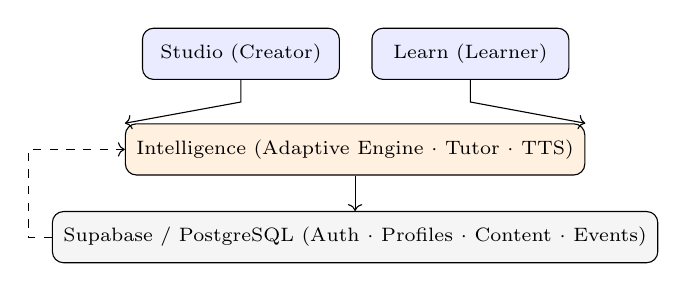
\begin{tikzpicture}[
  node distance=0.5cm,
  every node/.style={font=\scriptsize},
  surface/.style={rectangle, draw, rounded corners, minimum height=0.65cm,
    minimum width=2.5cm, inner sep=4pt, text centered},
  wide/.style={rectangle, draw, rounded corners, minimum height=0.65cm,
    minimum width=5.4cm, inner sep=4pt, text centered}
]
  \node[surface, fill=blue!8]  (studio) {Studio (Creator)};
  \node[surface, fill=blue!8, right=0.4cm of studio] (learn) {Learn (Learner)};
  \node[wide, fill=orange!12, below=0.55cm of studio, xshift=1.45cm] (intel)
        {Intelligence (Adaptive Engine $\cdot$ Tutor $\cdot$ TTS)};
  \node[wide, fill=gray!8, below=0.45cm of intel] (data)
        {Supabase / PostgreSQL (Auth $\cdot$ Profiles $\cdot$ Content $\cdot$ Events)};

  \draw[->] (studio.south) -- ++(0,-0.28) -- (intel.north west);
  \draw[->] (learn.south)  -- ++(0,-0.28) -- (intel.north east);
  \draw[->] (intel.south)  -- (data.north);
  \draw[->, dashed] (data.west) -- ++(-0.3,0) |- (intel.west);
\end{tikzpicture}
\caption{Sudar reference platform: three surfaces (Studio, Learn,
Intelligence) over a shared Supabase data layer. Solid arrows show
write/query flow; dashed arrow shows async profile update.}
\label{fig:arch}
\end{figure}


\subsection{Digital Learner Twin and Learner Model}
\label{sec:twin}

A persistent \textbf{Digital Learner Twin} is stored in
\texttt{learner\_profiles}. It includes: modality affinity scores
(per format, 0.0--1.0), learning pace and difficulty comfort,
behavioural signals (session duration, completion rate, streak), a
\texttt{preferences} field (JSONB) holding TTS voice selection,
response length preference (concise / one-line / detailed), and
modality preference notes, and an \texttt{ai\_tutor\_context} JSON
field holding known concepts, struggles, learning-style notes, goals,
and interaction summaries. This context is updated asynchronously from
tutor interactions and quiz outcomes. The design aligns with open
learner model principles \cite{bull2016} and supports personalisation
across courses and sessions. Crucially, the learner can inspect and
correct their own model at any time via the tutor's ``Your context''
panel, supporting metacognitive engagement \cite{zimmerman2002}.

\subsection{AI Tutor with Longitudinal Memory}
\label{sec:tutor}

The AI tutor, \textit{Sudar}, is both \emph{reactive}
(retrieval-augmented generation over course content to answer learner
questions) and \emph{proactive} (generating nudges when struggle or a
prolonged pause is inferred from behavioural signals). Every exchange
is logged in \texttt{ai\_interactions}. The tutor's system prompt
includes the learner's memory summary drawn from
\texttt{ai\_tutor\_context}, so responses reference prior struggles,
match the learner's preferred explanation style, and explicitly connect
new material to prior learning. Most AI in LMS implementations are
stateless \cite{zawacki2019}; Sudar is not.

Additional tutor capabilities include: a \textbf{text-selection
popup} that lets learners highlight any passage and invoke one of six
pre-built actions (``Explain this'', ``Give me an example'', ``Why
does this matter?'', ``Simplify this'', ``Summarise'', ``How does this
connect\ldots'') or a custom question; a \textbf{resizable overlay
panel}; \textbf{proactive nudges} on the dashboard and in the course
viewer with optional \emph{tap-to-reply} chips that forward to the same
tutor query pipeline; and a \textbf{generative block renderer} that allows the tutor
to respond with structured artefacts---quiz questions, course
recommendation cards, multi-step workflow trackers, and action
groups---enriching interaction beyond simple Q\&A.

\subsection{Modality-Agnostic Delivery}
\label{sec:modality}

Content is authored once. The delivery layer exposes a unified course
viewer with a modality switcher; \emph{which tabs are active depends
on course configuration} (e.g.\ video scenes and podcast dialogue are
optional fields in course settings). Learners always have Read, Listen,
Watch, Map, and Cards; Podcast appears when configured; Watch is only
fully active when the course includes generated or imported video
scenes; an optional \textbf{Play} link appears when a module provides a
SudarPlay asset. SCORM modules bypass the tab switcher and launch a
full-viewport package player.

\textbf{Text with Read-Along.} A server-side TTS read-along path
calls \texttt{/api/ai/generate-audio} per sentence, receiving neural
voice audio (Edge-TTS by default). Each sentence is highlighted in-place
as it plays, via \texttt{ReadingBodyWithSentences}. Telemetry includes
\texttt{read\_along\_start} / \texttt{read\_along\_complete} events.

\textbf{Listen (standalone audio TTS).} A dedicated Listen tab
(\texttt{AudioCard}) offers on-demand full-module TTS with optional
regeneration and learner voice preferences.

\textbf{Animated Video (Watch).} When \texttt{video\_scenes} are present,
the viewer renders scene-by-scene in-browser animation (kinetic,
word-reveal, fade, list). Richer video can be produced via the separate
SudarVid microservice and proxied by configuration. If no video is
available, the Watch tab remains disabled.

\textbf{Audio Podcast.} When \texttt{podcast\_dialogue} is configured,
the viewer presents a two-voice dialogue through \texttt{DialogueSegment[]}
with transcript and seek-by-segment playback.

\textbf{MindMap (SudarMind).} Generates an interactive concept map
on demand via \texttt{POST /api/ai/generate-mindmap} using a custom SVG
layout engine (B\'{e}zier edges, scope: module or course).

\textbf{Flashcards.} On-demand cards via \texttt{POST /api/ai/generate-flashcards},
supporting retrieval practice \cite{roediger2006,black1998}.

\textbf{SCORM.} Packages render in a sandboxed iframe with a
\texttt{postMessage} shim; scores and time write to
\texttt{learning\_events}. Extracted text can feed RAG for tutor
grounding.

Modality-aware delivery and learner affinity scores inform UX in Learn;
dual-coding principles \cite{mayer2009,clark2016} motivate the design
even where automation is partial.

\subsection{Adaptive Sequencing and Next-Best Action}
\label{sec:adaptive}

Learning paths support mandatory and optional courses and unlock rules.
For optional courses, the ordering is adapted by the Intelligence
engine from the learner profile and inferred knowledge gaps. A
next-best-action algorithm suggests the next course or module with a
human-readable explanation, surfacing required items and due-soon
deadlines. Formative assessment and struggle detection feed the learner
model \cite{black1998,roediger2006}.

Five quiz mode archetypes---standard closed-response, predict-then-learn,
confidence-tagged, scenario-fork, and peer-contrast---vary the
retrieval modality and support metacognitive calibration.

\subsection{Agent orchestration and auditability}
\label{sec:sudaragents}

Beyond conversational tutoring, Sudar exposes a gateway for \emph{bounded}
plans with a restricted tool catalogue: reads and scoped writes reuse the
Twin, \texttt{learning\_events}, and rollups, and each completed mission
records structured output plus tool traces in \texttt{agent\_runs}.
This is a design/implementation contribution: it operationalises
recommendation and light reflection loops aligned with formative practice
and calibration themes already emphasised above, without claims of new
empirical efficacy relative to unstructured chat. Org policy can disable
individual capabilities; integrators seeking a concise HTTP sketch can consult
\texttt{docs/ALP\_API.md} and \texttt{docs/AGENTS\_PLATFORM.md}.

% ---------------------------------------------------------------
\subsection{Plugin Architecture for Existing LMSs: The Adaptive
Learning Layer (ALP)}
\label{sec:alp}
% ---------------------------------------------------------------

The most novel architectural contribution is the \textbf{Adaptive
Learning Layer (ALP)}: a plugin layer that packages Sudar's
capabilities as independently deployable services for existing LMSs.
Organisations running Moodle, Canvas, Blackboard, or a proprietary LMS
need not abandon their investment to gain learner memory and adaptive
tutoring---ALP attaches these capabilities via APIs and event hooks.
Moodle~4.5 introduced a dedicated AI subsystem with a formal
separation between Provider plugins and Placement plugins
\cite{moodleai2025}; ALP is architecturally aligned with this model.

\paragraph{ALP reference API and roadmap plugin surfaces.}

\begin{enumerate}
  \item \textbf{SudarMemory (reference).} The foundational layer. Host
    LMS sends xAPI, SCORM outcomes, or webhooks to Sudar Learn's
    \texttt{/api/alp/events}; Sudar maintains a Digital Learner Twin per
    user. Vendor-packaged connectors are roadmap; the HTTP contract is
    implemented on Learn today.
  \item \textbf{SudarChat (reference).} Embeds the Sudar AI tutor via
    Learn's \texttt{/api/alp/tutor/query} and signed \texttt{/alp/embed}
    flows; Twin data is read from Supabase after org-scoped auth.
  \item \textbf{SudarStudio Embed (roadmap).} Target: ``Generate with
    AI'' inside the host LMS editor; today generation is authored in
    Sudar Studio/Learn rather than as installable LMS editor modules.
  \item \textbf{SudarRecommend (reference).} Next-best-action for the LMS
    dashboard via Learn's \texttt{/api/alp/next-action}; canonical scoring
    lives in Learn's \texttt{/api/intelligence/next-action}. No schema changes
    are required on the host database.
  \item \textbf{SudarAdapt (roadmap).} Target: LMS conditional activity
    integration for unlock/reorder; Sudar Learn already supports
    adaptive path ordering for Sudar-hosted paths.
  \item \textbf{SudarAgents (reference).} HTTP descriptors on Sudar Intelligence
    (\texttt{/api/agents/skills}, \texttt{/api/agents/alp-openapi.json})
    document the bounded orchestration surface for partner backends; see
    \texttt{docs/AGENTS\_PLATFORM.md}.
\end{enumerate}

\paragraph{Integration flow.}
Figure~\ref{fig:alp} illustrates the integration. The host LMS
continues to own content, enrolments, and grading. ALP sits alongside
it, enriching the experience without replacing infrastructure. No data
migration is required.

\paragraph{Reference implementation status.}
The repository provides authenticated HTTP endpoints on the Learn
application (e.g.\ \texttt{/api/alp/events}, \texttt{/api/alp/tutor/query},
\texttt{/api/alp/next-action}, embed-token helpers) with behaviour and
field mappings documented in \texttt{docs/ALP\_API.md}. Host LMSs can
call these without hosting Sudar's UI. Packaging the same contract as
distributable installable modules per vendor (Moodle, Canvas, etc.),
hardening for multi-tenant production, and mapping institutional user
identities, remain deployment engineering tasks rather than missing
core APIs.

\paragraph{Addressable scale.}
Moodle alone has over 500 million registered users across 233 countries
and holds approximately 28\% of the global LMS market
\cite{moodle2025stats}. ALP connectors for Moodle, Canvas, Blackboard,
and Sakai collectively address the largest possible deployment channel
for Sudar's intelligence layer without requiring a single institution
to change its LMS.

\paragraph{Positioning.}
We position ALP as an open \emph{reference architecture} and HTTP API
for memory-aware services alongside incumbent LMSs; related work
includes xAPI/LRS ecosystems, enterprise AI add-ons, and adaptive
extensions---we focus on an Apache-2.0 reference stack with explicit
trust and consent surfaces rather than claiming exclusive novelty.

\begin{figure}[t]
\centering
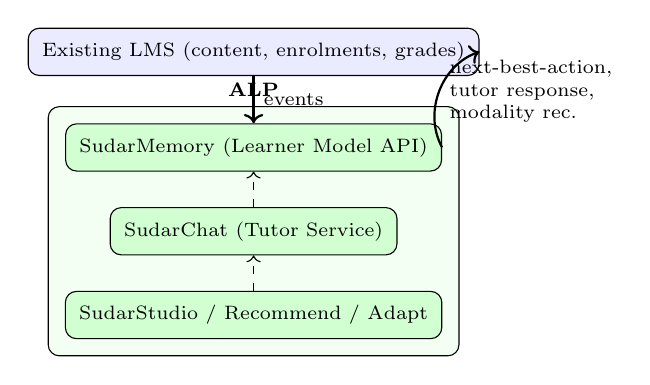
\begin{tikzpicture}[
  node distance=0.45cm,
  every node/.style={font=\scriptsize},
  box/.style={rectangle, draw, rounded corners, inner sep=5pt,
    minimum width=3.6cm, minimum height=0.6cm, text centered}
]
  \node[box, fill=blue!8] (lms)
    {Existing LMS (content, enrolments, grades)};
  \node[box, fill=green!18, below=0.6cm of lms] (api)
    {SudarMemory (Learner Model API)};
  \node[box, fill=green!18, below=0.45cm of api] (tutor)
    {SudarChat (Tutor Service)};
  \node[box, fill=green!18, below=0.45cm of tutor] (modal)
    {SudarStudio / Recommend / Adapt};

  \begin{scope}[on background layer]
    \node[draw, rounded corners, fill=green!5,
          fit=(api)(tutor)(modal),
          inner sep=6pt,
          label={[font=\scriptsize\bfseries]above:ALP}] {};
  \end{scope}

  \draw[->, thick] (lms.south) -- node[right, font=\scriptsize]{events} (api.north);
  \draw[->, dashed] (modal.north) -- (tutor.south);
  \draw[->, dashed] (tutor.north) -- (api.south);
  \draw[->, thick, bend left=50]
    (api.east) to node[right, font=\scriptsize, align=left]
      {next-best-action,\\tutor response,\\modality rec.}
    (lms.east);
\end{tikzpicture}
\caption{ALP integration architecture. The host LMS sends learning
events to SudarMemory; ALP returns next-best-action, tutor responses,
and modality recommendations. The LMS retains ownership of content and
enrolments.}
\label{fig:alp}
\end{figure}

\subsection{Open-Source Extensibility and the Modality Upgrade Path}
\label{sec:extensibility}

A distinguishing property of Sudar is that its modality delivery stack
is explicitly designed for community extension and backend substitution.
The \texttt{VideoScene[]}, \texttt{DialogueSegment[]}, and
\texttt{ModalityVariants} types are provider-agnostic interfaces; any
modality backend can be swapped without touching the delivery layer.

\paragraph{Video backend upgrade path.}
The current in-browser renderer delivers animated typographic video at
zero infrastructure cost. Organisations requiring higher production
value can connect any of the following backends to the same
\texttt{VideoScene[]} interface: \textbf{Higgsfield}
\cite{higgsfield2026}, a multi-model creative platform aggregating
Sora~2, Kling~2.6, and Google Veo~3.1 with cinema-grade camera
simulation; \textbf{Wan~2.1} \cite{wan2025} (Alibaba, MIT
open-source), a text-to-video suite from 1.3B to 14B parameters
enabling 480p generation on a consumer GPU; and
\textbf{HunyuanVideo} \cite{hunyuan2025} (Tencent, open-source), a
Diffusion Transformer model suited for instructor avatar generation in
corporate training contexts.

The principle is: Sudar is the authoring and delivery operating system;
the generation backend is a plugin. A school in Sub-Saharan Africa
self-hosts Wan~2.1 on a local GPU server at zero per-call cost. A
Fortune~500 L\&D team connects Higgsfield for cinematic course
introductions. The learner experience---the Digital Learner Twin,
adaptive sequencing, AI tutor, and modality switching---is identical.

\paragraph{Community extension patterns.}
The Apache-2.0 licence enables: new modality plugins (VR, AR, 3D simulation);
new LLM backends (any OpenAI-compatible API endpoint via environment
variable); new language and voice packs (Sarvam AI Indian English
neural voices are already integrated alongside Edge-TTS); and
vertical-specific forks for medical education, software engineering
bootcamps, and regulated-industry compliance.

\subsection{The Evolution of Sudar Intelligence}
\label{sec:intelligence}

The Intelligence layer described above reflects the current
implementation: reactive Q\&A via RAG, rule-based proactive nudges (with
structured follow-up \emph{choices} for client surfaces),
and a longitudinal memory updated from quiz outcomes and tutor
exchanges. This is a substantial advance over stateless LMS AI; it is
also, architecturally, only the beginning.

As the \texttt{learning\_events} table accumulates interaction data,
the Intelligence engine transitions from rule-based heuristics to
\emph{learned} intervention policies. The research frontier demonstrates
what becomes possible: reinforcement learning-driven ITS approaches can
improve intervention timing, adaptation, and learner persistence
relative to static rule-only tutoring policies.

Sudar's architecture anticipates this transition explicitly, with the
Digital Learner Twin and \texttt{learning\_events} stream serving as
the shared substrate for future first-party and community-built
Intelligence plugins: \textbf{SudarCoach} (career pathway advisor),
\textbf{SudarAssess} (item response theory psychometric layer),
\textbf{SudarSocial} (peer learning orchestrator),
\textbf{SudarCompliance} (automated evidence collection for regulated
industries), and \textbf{SudarTranslate} (real-time multilingual
delivery).

% ---------------------------------------------------------------
\section{Implementation and Reproducibility}
\label{sec:impl}
% ---------------------------------------------------------------

The reference platform is implemented with Next.js~15 (Studio, Learn;
TypeScript strict mode, App Router, Tailwind CSS),
Python~3.11+ FastAPI (Intelligence; async handlers, Pydantic v2), and
Supabase (PostgreSQL + pgvector, auth, storage). AI providers include
Together AI (primary; open-weight models), OpenAI, and Anthropic.
TTS uses Edge-TTS (default; zero cost, 40+ languages, 300+ voices)
with optional Sarvam AI Indian English neural voices. The schema and
event model are fully documented in the repository
(\texttt{ECOSYSTEM.md}, \texttt{RESEARCH\_FOUNDATION.md}).

Currently implemented: shared authentication and schema; course and
learning path CRUD and publish; document-to-course and SCORM~1.2
import; learner dashboard with streak, time-on-task, Sudar
recommendations, optional engagement surfaces (e.g.\ quests, coins,
achievements) where enabled, and upcoming deadlines; multimodal
course viewer as in Section~\ref{sec:modality} (read-along, Listen,
optional Watch and Podcast, Map, Cards, optional Play, SCORM); AI
tutor with longitudinal memory, RAG, text-selection popup, resizable
overlay, tap-to-reply proactive nudges, ``Your context'' live memory
panel, and generative block rendering; five quiz mode archetypes and
five lesson archetypes; next-best-action and adaptive path ordering;
learning paths with unlock rules, shareable public certificate pages,
browser print/save, and a server-generated PDF download route; optional
per-enrollment generative overlays with org policy and consent; Studio
governance and a technical trust pack for security reviews; compliance
view (overdue / at-risk / on-track) and email reminders
(cron); analytics rollups and risk signals (feature-flagged in
production); time per section in analytics; global search; server-side
sensitive-input guardrails on AI routes; and learner preferences. ALP
Learn proxies are implemented (Section~\ref{sec:alp}). Production
deployment is documented: Studio and Learn on Vercel; Intelligence on
Railway, Render, or Fly.io, with the Intelligence URL set in the apps.
The project is open source under the Apache-2.0 licence \cite{sudar2026}.

% ---------------------------------------------------------------
\section{Economic Accessibility: The Radical Cost Case}
\label{sec:economics}
% ---------------------------------------------------------------

The economic dimension of Sudar is not incidental to its design---it
is one of its three primary contributions.

\paragraph{Observed infrastructure cost.}
Operating Sudar at full engagement---10 courses generated, 20 learner
review sessions with AI tutor chat, adaptive personalisation, mindmap
generation, flashcard generation, and TTS narration---costs
approximately \textbf{\$0.20 per week} on the Together AI + Edge-TTS
stack. At organisational scale with 1,000 learners and 50 sessions per
month, the contrast is:

\begin{center}
\small
\begin{tabular}{@{}lrr@{}}
\toprule
Stack & Per month & Annual \\
\midrule
Sudar (Together AI + Edge-TTS) & \$21 & \$252 \\
GPT-4o + OpenAI TTS-1 & \$3,405 & \$40,860 \\
Claude 3.5 Sonnet + Azure TTS & \$3,735 & \$44,820 \\
Docebo (platform licence) & \$5,830+ & \$69,960+ \\
\bottomrule
\end{tabular}
\end{center}

At 10,000 learners, Sudar's open-weight stack costs approximately
\$210/month. The delta versus a closed-model stack---over \$400,000
per year---is the economic value of open-weight inference returned to
the institution rather than captured by AI API providers.

\paragraph{The inference cost collapse.}
AI inference costs have fallen approximately 1,000-fold from 2022 to
2026 at roughly 10$\times$ per year \cite{a16z2024llmflation}, driven
by GPU efficiency gains, software optimisation (vLLM, TensorRT-LLM),
Mixture-of-Experts architectures, and quantisation. GPT-3-class
performance costs \$0.06 per million tokens today versus \$60 in 2021.
The cost of delivering a world-class personalised tutor interaction to
one learner is now less than \$0.02 per month---below the cost of a
single SMS message. The economic argument against AI-native learning at
scale has expired.

\paragraph{The education access crisis.}
As of 2024, 251 million children and youth remain out of school
globally \cite{unesco2024}. 2.6 billion people remain offline
\cite{itu2024}, with mobile internet in Africa costing 14$\times$ more
than in Europe. An annual financing gap of \$39 billion exists for
basic education in low- and lower-middle-income countries through 2030
\cite{unesco2024}. The average corporate training spend per employee in
the United States is \$1,283 per year \cite{statista2023}; Sudar's
\emph{marginal} AI stack cost (\$0.21/user/month in our worksheet) is
\textbf{not comparable} to that all-in training benchmark---we include
it only to contrast order-of-magnitude \emph{LMS+AI API} stacks in the
table above, not to claim equivalent coverage.

High-end AI learning platforms priced at \$12--\$20 per user per month
are not deployable in this context. A platform whose full AI
infrastructure costs \$0.02 per learner per month---and whose stack is
open-source, self-hostable, and runnable on open-weight models---is.

% ---------------------------------------------------------------
\section{Evidence and Evaluation Strategy}
\label{sec:eval}
% ---------------------------------------------------------------

\paragraph{Research foundation.}
The design is evidence-informed. \texttt{RESEARCH\_FOUNDATION.md}
maps each capability to learning-science references: adaptive
instruction \cite{vanlehn2011,aleven2016}, dual coding
\cite{mayer2009,clark2016}, self-regulated learning
\cite{zimmerman2002}, formative assessment \cite{black1998,roediger2006},
intelligent tutoring \cite{self1988,vanlehn2011}, and learner
modelling \cite{bull2016,self1988}.

\paragraph{Scope of current claims.}
This is a system and architecture paper. Current claims are:
(a)~the platform implements a working reference deployment and the
subsystems we describe, with \emph{explicit} caveats for
course-dependent modalities, optional product layers, and ongoing LMS
packaging; (b)~each design choice is grounded in established
learning-science evidence; (c)~the ALP architecture addresses a gap in
LMS-agnostic, memory-aware services that commercial stacks rarely ship
as open, portable APIs; and
(d)~the economic cost structure has been empirically observed in
practice and validated against current provider pricing.

\paragraph{Pilot study.}
A pilot evaluation is planned, to be initiated after the current build
phase, and will be conducted in partnership with an organisational
partner to assess adoption, engagement, and early learning outcomes.
Results will be reported in a subsequent paper when available.

\paragraph{Future controlled studies.}
Plans include randomised or quasi-experimental comparisons of Sudar
versus a standard LMS on learning outcomes, learner satisfaction, and
time-to-competency, as well as studies isolating the contribution of
the longitudinal tutor memory component and the cost-per-outcome metric
versus incumbent platforms.

% ---------------------------------------------------------------
\section{Discussion}
\label{sec:discussion}
% ---------------------------------------------------------------

\paragraph{Limitations.}
Reference ALP HTTP endpoints and Learn-side proxies are implemented,
but \emph{packaging} and operating them as one-click add-ons in each
major LMS marketplace (and validating identity mapping in diverse SSO
environments) still requires per-institution work. Controlled efficacy
data are not yet available; claims about learning gains remain grounded
in the underlying learning-science evidence rather than
Sudar-specific trials. The Digital Learner Twin relies on inferred
signals that may not fully capture a learner's actual knowledge
state \cite{self1988,bull2016}. Edge-TTS uses Microsoft's voice
infrastructure under its terms; production deployments with paying
customers should plan licensed TTS. The predictive capabilities in
Section~\ref{sec:intelligence} require longitudinal data to learn
reliably; live systems today combine rules with heuristics.

\paragraph{Future work.}
Planned work includes: first-party or community LMS distributables
that wrap the same ALP contract; maturing analytics rollups and
scheduled jobs at scale; SudarFeed (short-form social feed) and deeper
SudarPlay integration; RL-style intervention policies; controlled
efficacy and cost-per-gain studies per \texttt{docs/PILOT\_PLAN.md};
SudarCoach, SudarAssess, and SudarCompliance-style intelligence
plugins; enterprise features (SSO, HRIS); and an offline-first
deployment path for low-connectivity settings.

% ---------------------------------------------------------------
\section{Conclusion}
\label{sec:conclusion}
% ---------------------------------------------------------------

We presented Sudar, an AI-native learning platform with three
contributions: (1)~a reference platform combining authoring, delivery,
and intelligence around a Digital Learner Twin, adaptive sequencing,
modality-agnostic delivery with course-dependent options, product
layers for policy/consent, engagement telemetry, and trust documentation,
and an AI tutor with longitudinal memory and proactive tap-to-reply
nudges; (2)~the Adaptive Learning Layer (ALP), an architecture and
reference API for deploying these capabilities alongside existing
LMSs---with the potential to reach the hundreds of millions
of Moodle, Canvas, Blackboard, and Sakai users \cite{moodle2025stats}
without requiring LMS replacement; and (3)~a demonstrated economic
model that reduces the infrastructure cost of AI-native personalised
learning to less than \$0.02 per learner per month, making it viable
at the scale of national education systems and accessible in contexts
where \$12--\$20/user/month platforms are structurally excluded.

The inference cost collapse is the macro condition that makes all of
this possible \cite{a16z2024llmflation}. Platforms built on open-weight
models and open-source infrastructure are positioned to pass this
economic gain directly to learners---particularly the 251 million
children currently out of school \cite{unesco2024} and the 2.6 billion
people currently offline \cite{itu2024}.

Together, these contributions offer a path to making adaptive,
memory-aware learning accessible both through a standalone platform and
as an augmentation of the LMSs that organisations already rely on. The
reference implementation is open source, grounded in a broad
learning-science evidence base
\cite{vanlehn2011,aleven2016,mayer2009,clark2016,zimmerman2002,%
gagne1985,bull2016,black1998,roediger2006}, and designed as a bedrock
upon which the community can build modalities, intelligence plugins,
and LMS connectors.

% ---------------------------------------------------------------
\section*{Acknowledgments}
% ---------------------------------------------------------------

The system and research are the author's project. The reference
implementation is available at
\url{https://github.com/Dhanikesh-Karunanithi/Sudar} with
documentation (\texttt{ECOSYSTEM.md}, \texttt{RESEARCH\_FOUNDATION.md},
\texttt{docs/sudar-memory.md}).

\begin{center}
\fbox{\parbox{0.9\columnwidth}{\small
\textbf{Call for collaboration.} Institutions, organisations, and
open-source contributors are invited to collaborate on pilots, plugin
integrations, and community extensions.
Contact: \texttt{connect@dhanikeshkarunanithi.com} or
\url{https://github.com/Dhanikesh-Karunanithi/Sudar}.
}}
\end{center}

% ---------------------------------------------------------------
\appendix
\section{Schema Summary}
% ---------------------------------------------------------------

Key tables for reproducibility:
\texttt{learner\_profiles} (Digital Learner Twin:
\texttt{ai\_tutor\_context}, \texttt{next\_best\_action}, modality
affinity scores, behavioural signals, \texttt{preferences} JSONB);
\texttt{learning\_events} (\texttt{event\_type}, payload, modality,
duration);
\texttt{ai\_interactions} (\texttt{user\_message},
\texttt{ai\_response}, \texttt{context\_used});
\texttt{enrollments} (path/course, progress, \texttt{due\_date},
optional \texttt{personalization\_overlays} JSONB);
\texttt{certifications}.
Full schema: \texttt{ECOSYSTEM.md} in the repository.

\section{Infrastructure Cost Reference}

\begin{center}
\small
\begin{tabular}{@{}p{3.2cm}rr@{}}
\toprule
Stack & /learner/mo & Annual (1k) \\
\midrule
Together AI 8B + Edge-TTS   & \$0.021  & \$252 \\
Together AI 70B + Edge-TTS  & \$0.105  & \$1,260 \\
GPT-4o + OpenAI TTS-1       & \$3.41   & \$40,860 \\
Claude 3.5 + Azure TTS      & \$3.74   & \$44,820 \\
Docebo (licence, low end)   & \$5.83   & \$69,960 \\
Sana Labs (est., min.\ 300) & $\approx$\$15 & $\approx$\$180k \\
\bottomrule
\end{tabular}
\end{center}
\noindent\small{AI infrastructure only; excludes hosting (Supabase free
tier: \$0; Pro: \$25/month).}

\section{Reproducibility and evaluation artefacts}
\noindent\small{Fill and version the cost assumptions in
\texttt{docs/research/COST\_WORKSHEET.md}; scope claims using
\texttt{docs/research/EVALUATION\_APPENDIX.md}; run pilots per
\texttt{docs/research/PILOT\_PROTOCOL.md}; extend
\texttt{scripts/benchmark-sudar.mjs} for automated latency/token
measurements when credentials are available.}

% ---------------------------------------------------------------
\bibliographystyle{plain}
\bibliography{references}
\end{document}
